\thispagestyle{plain}
\noindent% just to prevent indentation narrowing the line width for this line

\includegraphics[width=0.10\textwidth]{imagens/logo-unicamp}%
\begin{minipage}[b]{0.7\textwidth}
	\centering
	\textbf{UNIVERSIDADE ESTADUAL DE CAMPINAS} \\
\vspace{0.5cm}

\textbf{FACULDADE DE ODONTOLOGIA DE PIRACICABA}
\end{minipage}%

\includegraphics[width=0.10\textwidth]{imagens/logo-fop}

\vspace{4cm}
\begin{center}
	% O tamanho da fonte deve ser 16pt.
	% Deve-se utilizar caixa alta.
	{\Large\textsc{\autor}}
\end{center}
\vspace{4cm}
\begin{center}
	% O tamanho da fonte deve ser 16pt em negrito.
	% Deve-se utilizar caixa alta.
	{\Large\textbf{\textsc{\titulo}}}
\end{center}
\vfill
\begin{center}
	% O tamanho da fonte deve ser 12pt em negrito.
	% Deve-se utilizar caixa alta.
	\textbf{Piracicaba \\ \ano}
\end{center}





\cleardoublepage
% Folha de rosto


\thispagestyle{plain}


\begin{center}
	
	{\large\textbf{\textsc{\autor}}}
	
	
\end{center}
\vfill


\vfill
\begin{center}
	{\Large\textbf{\textsc{\titulo}}}
\end{center}
\vfill

\begin{flushright}
	\begin{minipage}[c]{.5\textwidth}
		\ifx\mestrado\undefined
		Tese apresentada à Faculdade de Odontologia de Piracicaba da Universidade Estadual de Campinas como parte dos requisitos para obtenção do título de \ifx\femaleAuthor\undefined
		Doutor
		\else
		Doutora
		\fi
		em \titulodoc{} na área de \areadoc . 
		\else
		Dissertação apresentada à Faculdade de Odontologia de Piracicaba da Universidade Estadual de Campinas como parte dos requisitos para obtenção do título de \ifx\femaleAuthor\undefined
		Mestre
		\else
		Mestra
		\fi
		em \titulodoc{} na área de \areadoc .
		\fi

		
		\end{minipage}
\end{flushright}
\vspace{.5cm}

\noindent
\textbf{Orientador\ifx\femaleOrientador\undefined
	\else
	a\fi: \orientador
}
\vspace{.25cm}

\ifx\coorientador\undefined
\else
\noindent
\textbf{Coorientador\ifx\femaleCoorientador\undefined
	\else
	a\fi: \coorientador
}
\vspace{.5cm}
\fi

\noindent
\begin{minipage}[c]{.5\textwidth}
	{\footnotesize\textsc{Este exemplar corresponde à versão final da
			\ifx\mestrado\undefined
			tese
			\else
			dissertação
			\fi
			defendida
			\ifx\femaleAuthor\undefined
			pelo aluno
			\else
			pela aluna
			\fi
			\autor,
			e orientada pel\ifx\femaleOrientador\undefined
			o\else
			a\fi{} Prof\ifx\femaleOrientador\undefined
			\else
			a\fi. Dr\ifx\femaleOrientador\undefined
			\else
			a\fi. \orientador.
		}}
	\end{minipage}
	\vspace{1cm}
	
	\noindent
	
	\vspace{.5cm}
	
	
	\vfill
	\begin{center}
		{\small\textbf{\textsc{ Piracicaba \\ \ano}}}
	\end{center}


\clearpage


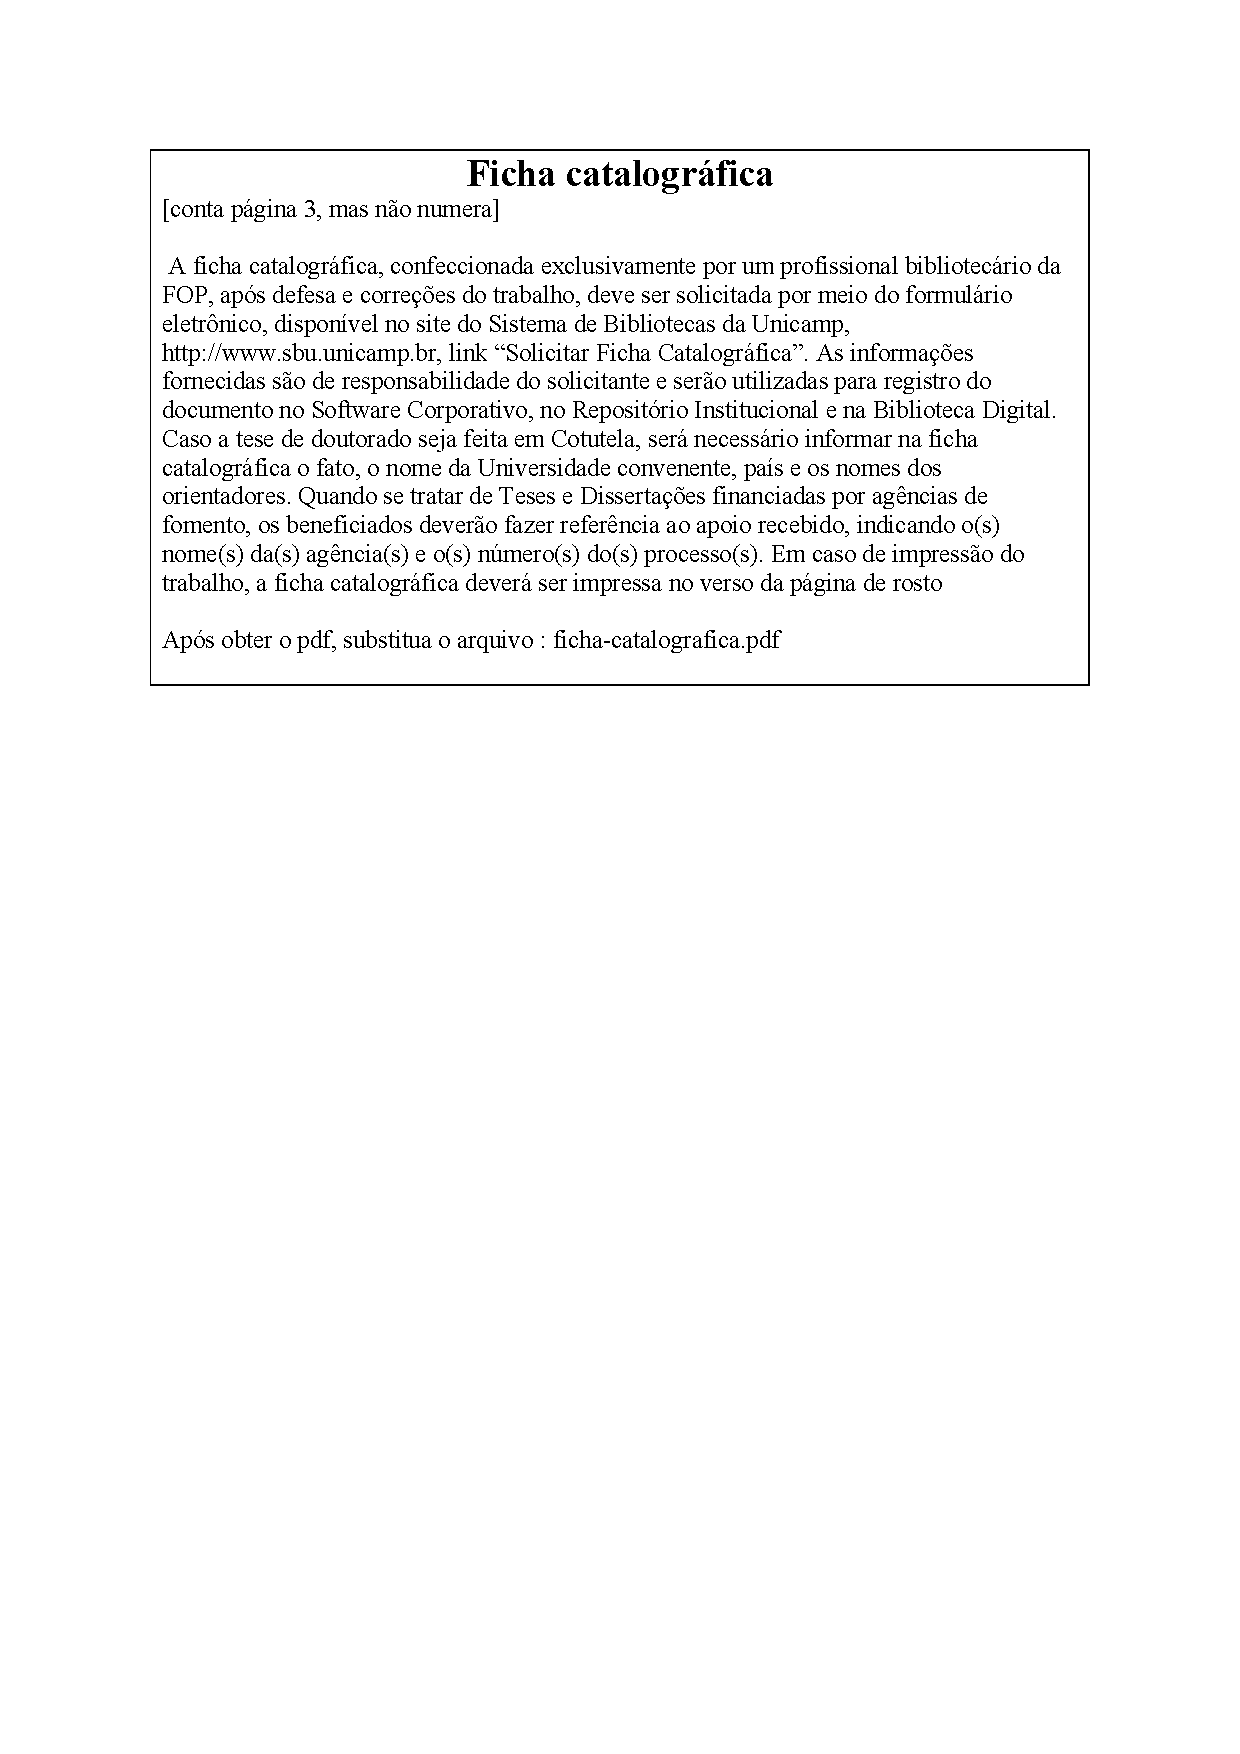
\includepdf{ficha-catalografica}

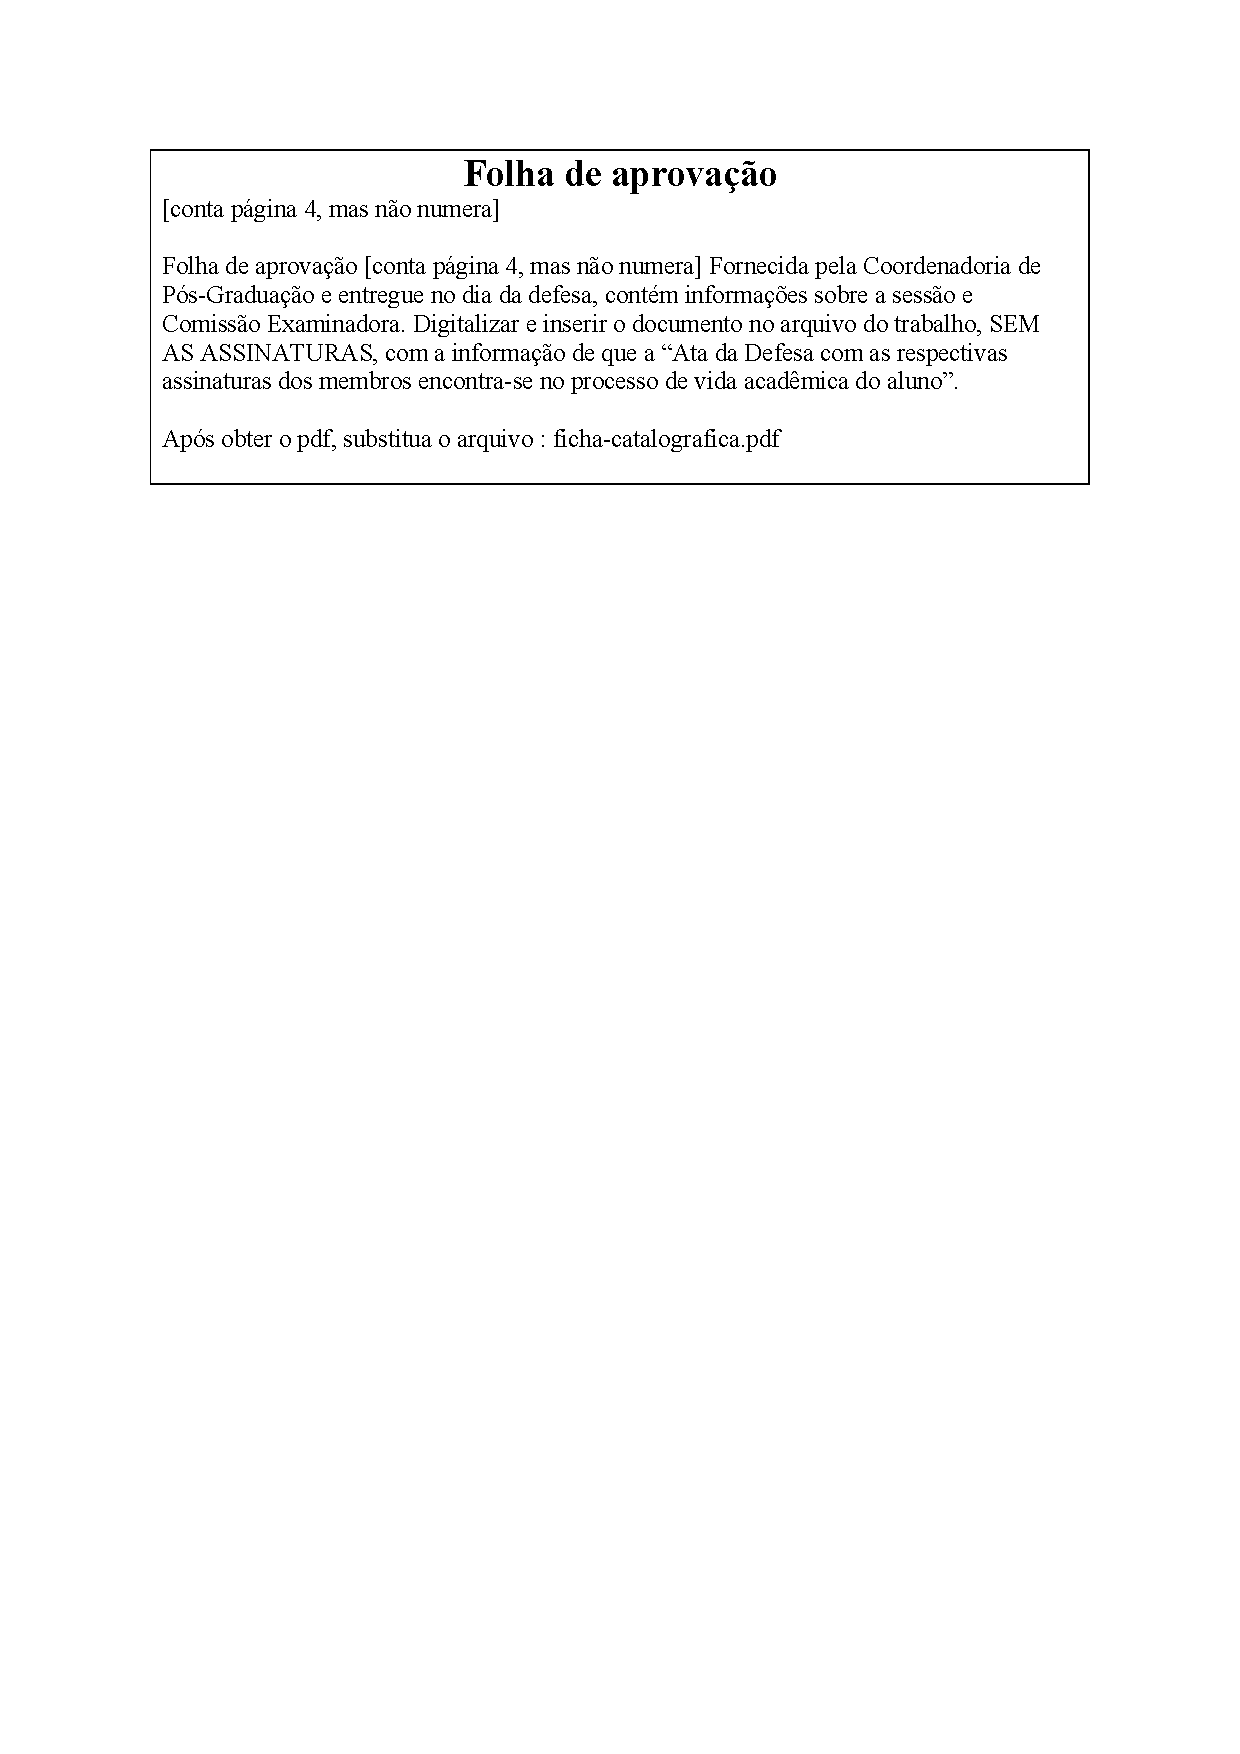
\includepdf{folha-de-aprovacao}
